\documentclass[UTF8]{ctexart}
\usepackage{graphicx}

\usepackage{ctex}
\CTEXsetup[format={\Large\bfseries}]{section}
\usepackage[top=28mm,bottom=28mm,left=15mm,right=15mm]{geometry}

\usepackage{fancyhdr}
\fancypagestyle{plain}{\pagestyle{fancy}}
\pagestyle{fancy}
\lhead{\kaishu 清华大学药学院药理毒理实验}
\newcommand{\numOfReport}[1]{\rhead{\kaishu 实验报告#1}}

\usepackage{fontspec}
\usepackage{wasysym}
\setCJKmainfont[AutoFakeBold={2}]{STZhongsong}
\setCJKmonofont{STZhongsong}

\usepackage{float}
\usepackage{booktabs}
\usepackage{tabularx}
\usepackage{array}
\usepackage{amsmath}
\usepackage{amsfonts}
\usepackage{amssymb}
\usepackage[figuresleft]{rotating}
\usepackage[para]{threeparttable}
\newcommand\info[2][40mm]{\underline{\makebox[#1][c]{#2}}}
\newcommand{\infoTable}[7]{
    \renewcommand\arraystretch{1.4}
    \begin{table}
        \begin{tabularx}{\textwidth}{
        >{\hsize=0.6\hsize\linewidth=\hsize}X
        >{\hsize=0.6\hsize\linewidth=\hsize}X
        >{\hsize=2.0\hsize\linewidth=\hsize}X
        >{\hsize=0.8\hsize\linewidth=\hsize}X
        }
            天气:\info[14mm]{#1} & 温度:\info[14mm]{#2 $^{\circ}\text{C}$} & 湿度:\info[14mm]{#3 $\%$} & 日期:#4\\
            姓名:\info[14mm]{#5} & 班级:\info[14mm]{#6} & 同组人:\info[70mm]{#7} & 
        \end{tabularx}
    \end{table}
}
\newcommand\columnC{\centering\arraybackslash}
\newcommand\columnL{\raggedright\arraybackslash}
\newcommand\columnR{\raggedleft\arraybackslash}

\usepackage{svg}
\usepackage{pdfpages}

\title{呋塞米对家兔的利尿作用研究}
\author{}
\numOfReport{九}

\begin{document}

\infoTable{阴}{10}{83}{11/13/2024}{何昱晖}{药3}{荣子健、马逸然、赵方一澜}
\date{}
\maketitle

\section{实验目的和原理}

\subsection{实验目的}

\begin{itemize}
    \item [1] 学习并掌握利尿剂的分类和作用原理;
    \item [2] 了解利尿实验的方法,观察呋塞米的利尿作用;
    \item [3] 熟悉并掌握家兔灌胃、麻醉、耳缘静脉注射、导尿管等实验操作。
\end{itemize}

\subsection{实验原理}

尿液的生成包括肾小球过滤、肾小管分泌和重吸收等三个过程,而影响肾小管重吸收的过程,可引起尿量的明显变化。利尿剂是指通过增加尿量,促进体内水分和电解质排出的药物。主要用于治疗心衰、肾衰竭、肾病综合症等引起的水肿,也可用于高血压。

临床常用的利尿药根据作用部位、化学结构、作用机制等可分为五类:

\begin{itemize}
    \item [1] 袢利尿剂:作用于\textbf{髓袢升支粗段},是最常用的一种利尿剂类型之一,代表药物是呋塞米;
    \item [2] 噻嗪类及类噻嗪类利尿剂:作用于远曲小管近端,常见代表药物为氢氯噻嗪等;
    \item [3] 碳酸酐酶抑制剂:主要作用于近曲小管,抑制碳酸酐酶活性,利尿作用弱,代表药物为乙酰唑胺;
    \item [4] 保钾利尿剂:主要作用于远曲小管远端和集合管,利尿效果相对较弱,但可以减少钾的排出量,代表药物为螺内酯、氨苯喋啶等;
    \item [5] 渗透性利尿剂:也称为脱水药,主要作用于髓袢及肾小管其他部位,代表药物为甘露醇。
\end{itemize}

呋塞米属高效利尿剂,又称为呋喃苯胺酸、速尿,主要作用于髓袢升支粗段的上皮细胞,竞争性抑制此段管腔膜上 $\text{Na}^+$-$\text{K}^+$-$2\text{Cl}^-$ 同向转运系统。抑制 $\text{Cl}^-$ 的主动转运,$\text{Na}^+$ 的重吸收也随之减少,导致管腔内 $\text{Na}^+$、$\text{Cl}^-$ 浓度增高,降低肾对尿液的稀释功能。同时,由于从髓袢升支重吸收到髓质间液 $\text{Na}^+$、$\text{Cl}^-$ 的量减少,影响其高渗透压状态的形成,使肾浓缩尿的功能降低,肾小管对 $\text{Na}^+$、$\text{Cl}^-$ 重吸收减少,$\text{Mg}^{2+}$、$\text{Ca}^{2+}$ 等二价阳离子重吸收也减少,由于大量 $\text{Na}^+$ 转运到远曲小管和集合管,促进 $\text{Na}^+$-$\text{K}^+$ 交换,故 $\text{K}^+$ 排出也增多,而 $\text{Cl}^-$ 不受离子交换影响,因而尿中 $\text{Cl}^-$ 多于 $\text{Na}^+$。因此,排出大量的电解质和水分而产生强大的利尿作用。

观察利尿药作用的实验方法通常包括:

\begin{itemize}
    \item [1] 直接从输尿管或膀胱收集尿液。实验动物通常采用狗、猫、家兔等较大动物。其优点为时间短、受外界影响小,但需要在麻醉或者手术等非生理状态下进行实验;
    \item [2] 「实验笼方法」:实验动物通常采用小鼠、大鼠,其优点为近生理状态,但实验环境影响大、实验时间长。
\end{itemize}

本实验采用第 1 种实验方法,通过收集家兔给药前、后单位时间内的尿量,计算单位时间内尿量增加毫升数,观察分析呋塞米的起效时间、作用强度及作用维持时间。

\section{实验材料}

\begin{itemize}
    \item 实验动物:家兔 1 只,体重 $2\sim 3\text{kg}$,雄性;
    \item 药品和试剂:舒泰 50 塞拉嗪麻醉剂、$1\%$ 呋塞米溶液、生理盐水、液体石蜡;
    \item 实验耗材:兔箱、兔手术台、兔开口器、灌胃器、导尿管、电子秤、量筒、烧杯、注射器、聚乙烯管、手术刀、组织剪、眼科剪、血管钳。
\end{itemize}

\section{实验方法}

\begin{itemize}
    \item [1] 取家兔 1 只,实验前禁食不禁水 $12\sim 24\text{h}$,称重;
    \item [2] 家兔灌胃:给予家兔灌胃生理盐水(20mL/kg)。本操作须二人完成,其中一人先将兔子固定,另一个人将开口器固定于兔口中,压住兔舌,然后将灌胃器从开口器的小孔中插入兔口中,再沿上颚壁顺食管方向送入胃中,插入动作要轻、慢,边插边密切关注动物的反应。为了防止误入气管,可将灌胃管的外端浸入水中,观察有无气泡产生。如有气泡逸出,则说明灌胃管误入气管,需重新插管。插好后将注射器连于灌胃管,慢慢将生理盐水推入,如很通畅,动物不挣扎,则说明已进入胃内。灌胃结束后,拔出胃管,取下开口器;

        \begin{itemize}
            \item [1] 此方法会对动物造成一定程度的机械性损伤和心理上的影响,为了尽量减少这些不良影响,必须熟练掌握灌胃技术;
            \item [2] 实验过程中须兔头及开口器,防止被咬伤;
            \item [3] 灌胃前须用灌胃管大致测量一下从口腔到胃内的位置长度,根据此距离估计灌胃管插入的深度,成年兔插入的深度一般约为 15cm;
            \item [4] 事先将灌胃管在水中或生理盐水中泡一下,使其更容易插入而不损伤食管;
            \item [5] 若灌胃不成功,则将家兔麻醉后耳缘静脉给予生理盐水(10mL/kg)。
        \end{itemize}

    \item [3] 家兔麻醉:灌胃成功后,家兔肌肉注射舒泰 50 联合塞拉嗪麻醉剂(给药剂量 $0.8\sim 1.3\text{mL}/\text{kg}\times 2\text{kg}$/只,观察家兔麻醉状态,记录麻醉时间。实验过程中需观察家兔麻醉状态,如需要可适量补加麻醉剂。
    \item [4] 尿道插管:将麻醉后的家兔仰卧位固定于兔台上(注意固定家兔时需要使用加热垫)。将导尿管尖端用液体石蜡润滑后,自家兔尿道缓缓插入,当观察到有尿液流出时,表示导尿管已经插入到膀胱内,再插入 $1\sim 2\text{cm}$(共插入 $8\sim 12\text{cm}$),用\textbf{胶布将导尿管与家兔身体固定}。计时,弃掉最初 5min 流出的尿液。用量筒收集随后的 20min 内尿量,记录收集尿液体积;
    \item [5] 耳缘静脉注射呋塞米溶液:自家兔耳缘静脉注射 $1\%$ 呋塞米(4mg/kg),随后收集并记录每 5min 内尿量,连续 6 次;
    \item [6] 家兔安乐死:实验结束后,自家兔大腿外侧再次缓慢注射舒泰 50 联合塞拉嗪麻醉剂(1mL/kg)进行安乐死,检查家兔心跳是否停止,以确认家兔死亡。
\end{itemize}

注意事项:

\begin{itemize}
    \item [1] 肌肉注射舒泰麻醉时需缓慢推注,边注射边观察家兔角膜反射、呼吸和肌肉松弛情况;
    \item [2] 插导尿管时动作应细致轻巧,切忌大力将膀胱插穿。如遇到阻碍的时候可以调整插入方向,以便导尿管能够顺利进入家兔膀胱内;
    \item [3] 静注呋塞米溶液后,一般 3min 即发挥利尿作用,如无尿液滴出,应检查导管内是否凝血或导尿管口堵住,缓慢转动或前后移动导尿管位置,直到尿液流出;
    \item [4] 实验过程中应注意动物的保温。
\end{itemize}

\section{实验结果}

\begin{table}[H]
    \centering
    \begin{threeparttable}[b]

        \caption{单位时间内尿量增加毫升数}
        \quad
        \begin{tabularx}{\textwidth}{
            >{\columnC\hsize=1\hsize\linewidth=\hsize}X
            >{\columnC\hsize=1\hsize\linewidth=\hsize}X
        }
            \toprule[1.5pt]
            组号 & 单位时间尿量增加毫升数\\
            \midrule
            1 & $1.65\pm 1.73$ \\
            2 & $3.19\pm 0.94$ \\
            3 & $1.35\pm 0.72$ \\
            4 & $2.85\pm 0.95$ \\
            5 & $0.85\pm 0.59$ \\
            6 & $0.16\pm 0.58$ \\
        \end{tabularx}

    \end{threeparttable}
\end{table}

\begin{figure}[H]
    \centering
    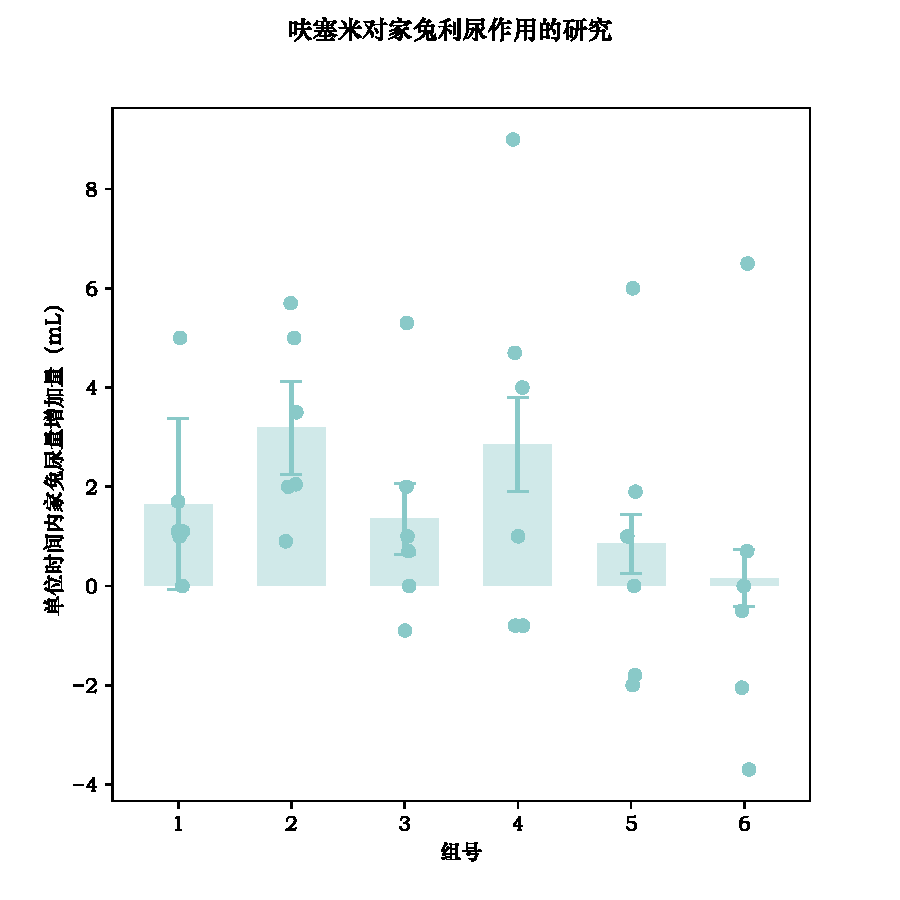
\includegraphics{figure-9_svg.pdf}
    \caption{呋塞米对家兔的利尿作用研究}
\end{figure}

\section{课后思考题}

\begin{itemize}
    \item [1] 简述利尿药的分类及作用机制

    \begin{itemize}
        \item [1] 袢利尿剂:作用于\textbf{髓袢升支粗段},是最常用的一种利尿剂类型之一,代表药物是呋塞米;
        \item [2] 噻嗪类及类噻嗪类利尿剂:作用于远曲小管近端,常见代表药物为氢氯噻嗪等;
        \item [3] 碳酸酐酶抑制剂:主要作用于近曲小管,抑制碳酸酐酶活性,利尿作用弱,代表药物为乙酰唑胺;
        \item [4] 保钾利尿剂:主要作用于远曲小管远端和集合管,利尿效果相对较弱,但可以减少钾的排出量,代表药物为螺内酯、氨苯喋啶等;
        \item [5] 渗透性利尿剂:也称为脱水药,主要作用于髓袢及肾小管其他部位,代表药物为甘露醇。
    \end{itemize}

    \item [2] 针对呋塞米的作用机制,推测其可能出现的副作用及其原因

        长期使用呋塞米可能造成电解质紊乱,低血钾、低血钠。原因是呋塞米使得大量的钾和钠从人体排出
\end{itemize}

\end{document}
